\documentclass[11pt]{article}

\usepackage[T1]{fontenc}
\usepackage{geometry}
\usepackage{amsmath, amssymb, amsthm}
\usepackage[scr]{rsfso}
\usepackage[%
    hidealllines=true,%
    innerbottommargin=15,%
    nobreak=true,%
]{mdframed}
\usepackage{xcolor}
\usepackage{graphicx}
\usepackage{fancyhdr}
\usepackage{hyperref}

\geometry{a4paper, margin=1in, headheight=14pt}

\pagestyle{fancy}
\fancyhf{}
\renewcommand\headrulewidth{0.4pt}
\fancyhead[L]{\scshape MA3103}
\fancyhead[R]{\scshape \leftmark}
\rfoot{\footnotesize\it Updated on \today}
\cfoot{\thepage}

\newcommand{\C}{\mathbb{C}}
\newcommand{\R}{\mathbb{R}}
\newcommand{\Q}{\mathbb{Q}}
\newcommand{\Z}{\mathbb{Z}}
\newcommand{\N}{\mathbb{N}}

\newmdtheoremenv[%
    backgroundcolor=blue!10!white,%
]{theorem}{Theorem}[section]
\newmdtheoremenv[%
    backgroundcolor=violet!10!white,%
]{corollary}{Corollary}[theorem]
\newmdtheoremenv[%
    backgroundcolor=teal!10!white,%
]{lemma}[theorem]{Lemma}

\theoremstyle{definition}
\newmdtheoremenv[%
    backgroundcolor=green!10!white,%
]{definition}{Definition}[section]
\newmdtheoremenv[%
    backgroundcolor=red!10!white,%
]{exercise}{Exercise}[section]

\theoremstyle{remark}
\newtheorem*{remark}{Remark}
\newtheorem*{example}{Example}
\newtheorem*{solution}{Solution}

\surroundwithmdframed[%
    linecolor=black!20!white,%
    hidealllines=false,%
    innertopmargin=5,%
    innerbottommargin=10,%
    skipabove=0,%
    skipbelow=0,%
]{example}

\numberwithin{equation}{section}

\title{
    \Large\textsc{MA3103} \\
    \Huge \textbf{Introduction to Graph Theory and Combinatorics} \\
    \vspace{5pt}
    \Large{Autumn 2021}
}
\author{
    \large Satvik Saha
    \\\textsc{\small 19MS154}
}
\date{\normalsize
    \textit{Indian Institute of Science Education and Research, Kolkata, \\
    Mohanpur, West Bengal, 741246, India.} \\
}

\begin{document}
    \maketitle

    \tableofcontents

    \section{Introduction}
    
    \subsection{The Seven Bridges of K\"onigsberg}
    
    The diagram below depicts a region in the city of K\"onigsberg, Prussia. There
    are two islands, connected with the mainland and to each other via seven bridges.
    The Seven Bridges Problem is posed as follows: is it possible to walk through the
    entire city, visiting each one of the four landmasses by crossing each of the
    bridges exactly once?

    \begin{center}
        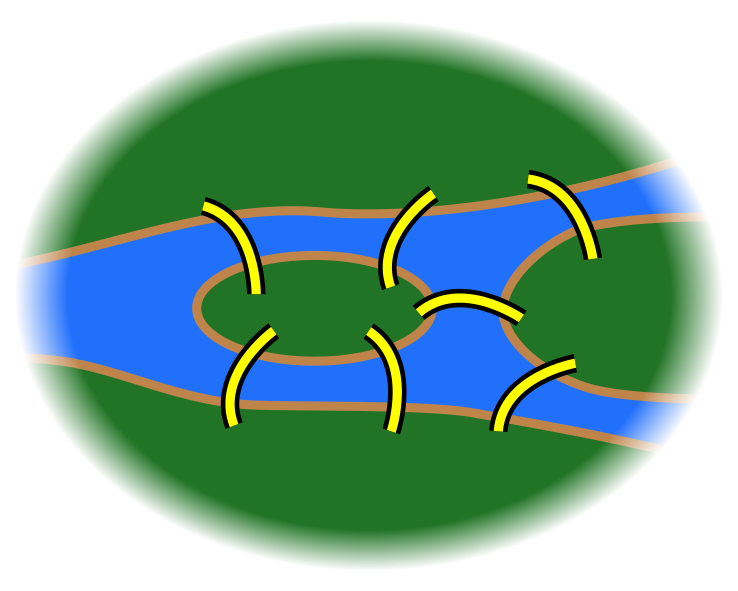
\includegraphics[width=0.6\textwidth]{7_bridges.png}
    \end{center}

    Leonhard Euler showed that this is impossible; no such walk exists. The
    techniques he developed in doing so laid the foundations of \textit{graph
    theory}.

    The first thing to note is that the exact shape of the walk/trail is immaterial;
    all that matters is the sequence of landmasses visited and bridges crossed. Thus,
    each landmass can be compacted to a single point or \textit{vertex}, and each
    bridge a line or \textit{edge} connecting two such points. The resulting figure
    is a graph. Note that the orientations or placements of the points and lines are
    irrelevant, as long as the connections are undisturbed.

    \begin{center}
        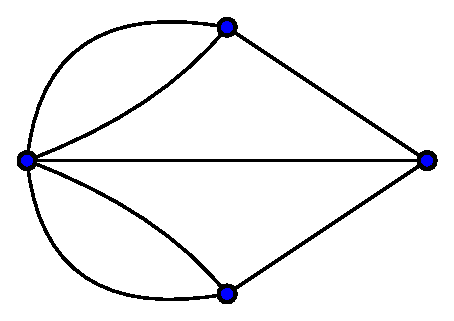
\includegraphics[width=0.5\textwidth]{7_bridges_graph.eps}
    \end{center}

    Now, examine a landmass which is on the trail but is neither our starting point,
    nor our ending point. In order to reach this landmass, we must enter via a bridge; but
    we cannot stay in the landmass, so we must leave via another a bridge. Thus, for
    each time we pass through this landmass, we can cross off two bridges joined to
    it. Once we are done, no bridge may remain unused; this means that we must have
    started with an even number of bridges joined to this landmass.

    However, all four vertices in our graph connect to an odd number of edges. Since
    we require at least two vertices to act as intermediate points on our path, the
    desired walk is impossible.

    \subsection{Basic definitions}
    \begin{definition}
        A graph $G(V, E)$ is an ordered pair of the set of vertices $V$ and the set
        of edges $E$.
    \end{definition}
    \begin{definition}
        A simple graph is undirected, unweighted, and contains no self-loops or
        multiple edges joining vertices.
    \end{definition}
    \begin{definition}
        For a simple undirected graph, the set of edges $E$ consists of two-element
        subsets of the set of vertices $V$.
        \begin{remark}
            For a directed, unweighted graph, the set of edges $E$ consists of ordered
            pairs of elements from the set of vertices $V$.
        \end{remark}
    \end{definition}
    \begin{definition}
        A vertex is incident to an edge if that edge joins that vertex.
    \end{definition}
    \begin{definition}
        Two vertices are adjacent if there exists an edge connecting them.
        Two edges are adjacent if they connect to a common vertex.
    \end{definition}
    \begin{definition}
        The neighbours of a vertex consist of all vertices adjacent to it.
        The neighbours of an edge consist of all edges adjacent to it.

        The number of neighbours of a vertex is called the degree of that vertex.
    \end{definition}

    \begin{definition}
        A complete graph is such that every pair of vertices is connected by an
        edge. The complete (simple) graph of $n$ vertices is denoted by $K_n$.
    \end{definition}

    \subsection{Some principles}
    
    \begin{lemma}[Pigeonhole Principle]
        If $n + 1$ objects are placed in $n$ boxes, then we can fin a box containing
        at least $2$ objects.
    \end{lemma}
    \begin{proof}
        If every box contains at most $1$ objects, then the total number of objects
        falls short.
    \end{proof}

    \begin{theorem}
        There are no simple graphs where the degrees of all vertices are distinct.
    \end{theorem}
    \begin{proof}
        Let $G(V, E)$ be a simple graph with $n$ vertices. The degrees of each of
        these vertices must be an integer among $0, 1, \dots, n - 1$. We now consider
        two cases. \\

        \textbf{Case I}: There is a vertex of degree $0$. Thus, this vertex is
        adjacent to no other vertex, which means that no vertex can have the full
        degree $n - 1$. This means that the remaining vertices have degrees among $1,
        2, \dots, n - 2$, i.e.\ $n - 2$ choices of degree for $n - 1$ vertices.

        \textbf{Case II}: There is no vertex of degree $0$. Thus, the vertices have
        degrees among $1, 2, \dots, n - 1$, i.e.\ $n - 1$ choices of degree for $n$
        vertices. \\

        In either case, the Pigeonhole Principle forces at least two vertices to
        share the same degree.
    \end{proof}

    \begin{lemma}[Strong Pigeonhole Principle]
        Let $q_1, q_2, \dots, q_n$ be positive integers. If \[
            N = q_1 + \dots + q_n - n + 1
        \] objects are placed in $n$ boxes, then we can find a box $i$ containing at
        least $q_i$ objects.
    \end{lemma}
    \begin{proof}
        If every box $i$ contains at most $q_i - 1$ objects, then the total number of
        objects falls short. \[
            N \leq (q_1 - 1) + \dots + (q_n - 1) = q_1 + \dots + q_n - n = N - 1 \qedhere
        \] 
    \end{proof}

    \begin{theorem}
        The sum of the degrees of all vertices in a simple graph is twice the number
        of its edges. 
    \end{theorem}
    \begin{proof}
        Let $G((V, E)$ be a simple graph. 
        Define the incidence function $I\colon E \times V \to \{0, 1\}$, such that
        $I(e, v) = 1$ if $e$ and $v$ are incident, $0$ otherwise. We perform the
        double counting, \[
            \sum_{v\in V}\sum_{e \in E} I(e, v) = \sum_{e \in E}\sum_{v \in V} I(e,
            v).
        \] Now, the number of edges incident to a vertex is simply its degree, so
        $\sum_{e \in E} I(e, v) = d(v)$. Also, every edge is incident to exactly two
        vertices, so $\sum_{v \in V} I(e, v) = 2$. Thus, we have \[
            \sum_{v \in V} d(v) = 2 |E|. \qedhere
        \] 
    \end{proof}

    \begin{lemma}[Inclusion-Exclusion Principle]
        For finite sets $A_1, A_2, \dots, A_n$, the number of elements in their union
        is given by \[
            \sum_{i=1}^n |A_i| - \sum_{1 \leq i < j \leq n} |A_i\cap A_j| +
            \sum_{1 \leq i < j < k \leq n} |A_i \cap A_j\cap A_k| - \dots + 
            (-1)^{n-1} \left|A_1\cap\cdots\cap A_n\right|.
        \] 
    \end{lemma}

    \begin{theorem}
        There are $2^{\binom{n}{2}}$ simple graphs with $n$ vertices.
    \end{theorem}
    \begin{exercise}
        How many simple graphs are there with $n$ vertices and $m$ edges?
    \end{exercise}
    \begin{theorem}
        Let $n, k \in \N$ such that $n > 3$ and $n / 2 < k < n$. Let there be $n$
        points on a plane such that no three points are collinear. If every point is
        connected to at least $k$ other points by segments, then there must be at
        least three segments forming a triangle.
    \end{theorem}
    \begin{proof}
        Consider a graph $G(V, E)$ with $n$ vertices, such that every vertex has
        degree at least $k$. Pick an edge, say $\{x, y\}$, and let $A$ be the
        neighbours of $x$ apart from $y$, $B$ be the neighbours of $y$ apart from
        $x$. Note that $A$, $B$ have at least $k - 1$ elements each. Suppose that $A
        \cap B = \emptyset$, i.e.\ the edge $\{x, y\}$ doe not form a triangle. Thus,
        \[
            |A\cup B| = |A| + |B| - |A \cap B| \geq 2(k - 1).
        \] However, $|A\cup B| \leq n - 2$, hence $n \geq 2k$, or $k \leq n / 2$.
        This is a contradiction.
    \end{proof}
    \begin{remark}
        We have shown that \emph{every} segment is part of a triangle. The number of
        segments here is \[
            |E| \geq n k > \frac{n^2}{4}.
        \] 
    \end{remark}
    \begin{exercise}
        Is the condition $|E| > n^2 / 4$ sufficient to ensure the existence of a triangle?
    \end{exercise}

    \begin{lemma}[Cauchy-Schwarz]
        Let $a_1, \dots, a_n$ and $b_1, \dots, b_n$ be positive reals. Then, \[
            (a_1^2 + \dots + a_n^2) (b_1^2 + \dots + b_n^2) \geq (a_1b_1 + \dots +
            a_nb_n)^2.
        \] Equality holds if and only if every $a_i = \lambda b_i$ for some fixed
        real $\lambda$.
    \end{lemma}

    \begin{theorem}[Mantel]
        In a simple graph with $n$ vertices, the condition $|E| > n^2 / 4$ is
        sufficient to ensure the existence of a triangle.
    \end{theorem}
    \begin{proof}
        Let $G$ be a simple graph with $n$ vertices which is triangle-free. Thus, for
        any edge $\{x, y\} \in E$, the neighbour sets $A$ and $B$ of $x$ and $y$
        intersect at no vertex. Thus, we can write \[
            d(x) + d(y) = |A \cup B| \leq n.
        \] Sum this over all possible edges. On the right, we have $n|E|$. On the
        left, we have the sum \[
            \sum_{x \in V} d(x)^2 \geq \frac{1}{n} \left(\sum_{x \in V} d(x)\right)^2
            \geq \frac{1}{n} \cdot 4|E|^2
        \] This gives \[
            \frac{4|E|^2}{n} \leq n |E|, \qquad |E| \leq \frac{n^2}{4}. \qedhere
        \] 
    \end{proof}
    \begin{example}
        Consider a circle, with 21 points on its circumference. It follows that among
        the angles subtended by these points at the center, at most 110 are greater
        than $2\pi / 3$. \\

        Note that there are $\binom{21}{2} = 210$ angles. Furthermore, given any 3
        points on the circle (forming a triangle), all three angles subtended by them
        cannot be greater than $2\pi / 3$. Construct a graph with these $n = 21$
        points as vertices, such that two vertices are connected by an edge if and
        only if the angle subtended by them is greater than $2\pi / 3$.  Now, note
        that $n^2 / 4 = 110.25$, thus if there are more than $110$ edges, there must
        exist a triangle of vertices in which all three angles are greater than $2\pi
        / 3$ -- a contradiction!
    \end{example}

    \subsection{Bipartite graphs}
    \begin{definition}
        A graph $G(V, E)$ is called bipartite if the vertex set $V$ can be
        partitioned into 2 parts $V_1$, $V_2$ such that every edge in $E$ joins a
        vertex of $V_1$ to a vertex of $V_2$. In other words, there exists a 2-
        colouring of the vertices such that no edge connects two vertices of the same
        colour.

        \begin{remark}
            The sum of the degree of the vertices in one part is exactly equal to
            the number of edges, which in turn is equal to the sum of the degrees of
            the vertices in the other part.
        \end{remark}
    \end{definition}

    \begin{definition}
        A complete bipartite graph is such that each vertex in one part is connected
        to every vertex in the other part. Such a graph is denoted by $K_{m,n}$,
        where the parts have $m$ and $n$ vertices respectively.

        \begin{remark}
            The total number of edges must be the product of the numbers of vertices
            in each part.
        \end{remark}
    \end{definition}

    \begin{definition}
        A set of vertices (or edges) in a graph is called independent if no two
        elements in that set are adjacent.
    \end{definition}

    \begin{lemma}
        A bipartite graph is triangle free.
    \end{lemma}

    \begin{corollary}
        If we choose even $n$, we can achieve a triangle free graph with $n^2 / 4$
        edges, namely $K_{n / 2, n / 2}$. Similarly, if $n$ is odd but $\lfloor n^2 /
        4\rfloor$ factors into natural numbers $\lceil n / 2\rceil$ and $\lfloor n /
        2 \rfloor$, then $K_{\lceil n / 2\rceil, \lfloor n / 2 \rfloor}$ achieves the
        upper bound again.
    \end{corollary}
    
    \begin{lemma}
        An $r$-partite graph is $K_{r + 1}$ free.
    \end{lemma}

    \begin{exercise}
        Consider a complete $r$-partite graph on $n$ vertices. What is the maximum
        number of edges possible?
        \begin{solution}
            Consider $K_{n_1, \dots, n_r}$, where $n = n_1 + \dots + n_r$. The number
            of edges is \[
                |E| = \sum_{i < j} n_i n_j.
            \] Cauchy-Schwarz gives \[
                n^2 = \sum_{i} n_i^2 + 2\sum_{i < j} n_i n_j \geq \frac{n^2}{r} +
                2|E|.
            \] Thus, \[
                |E| \leq \frac{n^2}{2}\left(1 - \frac{1}{r}\right).
            \] Equality is achieved when $n_1 = \dots = n_r$.
        \end{solution}
    \end{exercise}

    \begin{definition}
        The complete $r$-partite graph $K_{n_1, \dots, n_r}$ on $n$ vertices, such
        that $|n_i - n_j| \leq 1$ for all $i, j$ is called Turan's graph, $T_{n, r}$.
    \end{definition}

    \begin{theorem}[Turan's Theorem]
        The number of edges in a $K_{r + 1}$ free graph on $n$ vertices is at most \[
            |E(T_{n, r})| = \frac{n^2}{2} \left(1 - \frac{1}{r}\right).
        \]
    \end{theorem}
    \begin{proof}
        Fix $r$; we prove the theorem by induction on $n$. The base case $n = 2$ has
        already been shown. Suppose that this holds for all $K_{r + 1}$ free graphs
        with less than $n$ vertices. Note that whenever $n \leq r$, the claim is
        obvious, since \[
            |E| \leq \frac{n (n - 1)}{2} \leq \frac{n^2}{2}\left(1 -
            \frac{1}{r}\right).
        \] Otherwise, we have $n \geq n + 1$. Let $G$ have the maximum number of
        edges such that it is $K_{r + 1}$ free. We argue that $G$ must contain $K_r$;
        if not, there is still scope for adding edges. Call the vertices in this
        subset $A$, and the remaining vertices $B$. Clearly, $|A| = r$ and $|B| = n -
        r$. Set $e_A$ equal to the number of edges within $A$, $e_B$ the number of
        edges within $B$, and $e_{AB}$ the number of edges between $A$ and $B$. We
        must have $|E| = e_A + e_B + e_B$. Now, $A$ has the structure of $K_r$, so
        $e_A = r(r - 1) / 2$. Since the structure of $B$ is $K_{r + 1}$ free, we can
        apply the induction hypothesis on it, giving $e_{B} \leq (n - r)^2(r - 1) /
        2r$. Finally, no vertex in $B$ can be connected to every vertex in $A$, so we
        have $e_{AB} \leq (r - 1)(n - r)$. Adding everything together, 
        \begin{align*}
            |E| &\leq \frac{r (r - 1)}{2} + \frac{(n - r)^2(r - 1)}{2r} + (r - 1)(n -
            r) \\
            &= \frac{1}{2} \left[r^2 + (n - r)^2 + 2r(n - r)\right]\frac{r - 1}{r} \\
            &= \frac{n^2}{2}\left(1 - \frac{1}{r}\right).
        \end{align*}
        Note that for equality to hold, we require every vertex in $B$ to be
        connected to $r - 1$ vertices in $A$. This means that $B$ is the Turan's
        graph $T_{n - r, r}$, so $G$ is the Turan's graph $T_{n, r}$.
    \end{proof}

    \begin{example}
        We give a second proof of Mantel's Theorem. Let $G$ be a triangle free graph
        on $n$ vertices. Let $A$ be an independent set of $G$, and let $B$ be the set
        of remaining vertices. Furthermore, let $A$ be a \emph{largest} independent
        set of $G$. Now note that in a triangle free graph, the neighbouring set of
        any vertex must be an independent set. This gives an upper bound of $|A|$ on
        the degree of any vertex. Also note that given an arbitrary edge, one of its
        endpoints must lie in $B$ (both endpoints cannot lie in $A$ since it is an
        independent set). This forces \[
            |E| \leq \sum_{x \in B} d(x) \leq |A| |B| \leq \frac{1}{4}(|A| + |B|)^2 =
            \frac{n^2}{4}.
        \] 
        Now, note that for equality in the first case, we require no edges in $B$,
        i.e.\ $B$ must be independent. This forces $G$ to be bipartite. For the
        second equality, we need every vertex in $B$ to have the full degree $|A|$,
        so $G$ is a complete bipartite graph. For the third equality, we demand $|A|
        = |B|$, so $G = T_{n, 2}$.
    \end{example}

    \subsection{Subgraphs}
    \begin{definition}
        Let $G(V, E)$ be a graph. We say that $G'(V', E')$ is a subgraph of $G(V, E)$
        if $V' \subseteq V$ and $E' \subseteq E$. We write $G' \subseteq G$.
    \end{definition}

    \begin{definition}
        The subgraph $G'$ induced by a set of vertices $V' \subseteq V$ is such that
        $G'$ contains all the edges of $G$ that connect vertices from $V'$. We write
        $G' = G[V']$.
    \end{definition}

    \begin{definition}
        The subgraph $G'$ spans its parent $G$ if the vertex sets $V' = V$.
    \end{definition}

    \begin{definition}
        A $k$-clique of $G$ is an induced subgraph on $k$ vertices which is complete.
    \end{definition}

    \begin{definition}
        The Ramsey number $R(s, t)$ is the least positive integer for which every
        complete graph on that many vertices, with its edges coloured in red and
        blue, must contain either a red $s$-clique or a blue $t$-clique.
    \end{definition}
    \begin{example}
        We can see that $R(s, t) = R(t, s)$, $R(1, r) = 1$, $R(2, r) = r$.
    \end{example}
    \begin{example}
        We can show that $R(3, 3) = 6$. Indeed, every colouring of $K_6$ must contain
        at least \emph{two} monochromatic triangles.
    \end{example}
    \begin{example}
        Consider any graph $G$ on $6$ vertices. Construct a new graph $G'$ on $6$
        vertices where two vertices are joined by a red edge if there exists a
        corresponding edge in $G$, and blue if not. Thus, $G'$ is a 2-coloured
        complete graph and hence contains a monochromatic triangle. This means that
        there are 3 vertices in $G$ where either all of them are connected to each
        other, or none of them are.
    \end{example}
    \begin{lemma}
        The number $R(s, t)$ is the smallest positive integer such that any graph on
        $R(s, t)$ vertices contains either an independent set of size $s$, or a
        $t$-clique.
    \end{lemma}

    \begin{theorem}[Ramsey Theorem]
        The Ramsey number $R(s, t)$ is always finite.
    \end{theorem}
    \begin{proof}
        We show this for all $s, t \geq 3$ by induction on $s + t$. Note that when $s
        + t = 6$, we know that $R(1, 5)$, $R(2, 4)$, $R(3, 3)$ are all finite.
        Furthermore, $R(s, 1) = R(1, t) = 1$. Suppose that $R(s - 1, t)$ and $R(s, t
        - 1)$ are both finite; we claim that $R(s, t) < R(s - 1, t) + R(s, t - 1)$.
        Without loss of generality, let $s \geq t$. Consider a complete graph $K_n$ on
        $R(s - 1, t) + R(s, t - 1) = n$ vertices. Choose a vertex $v$, and let $V_R$
        be the set of its neighbours connected by red edges, $V_B$ be the neighbours
        connected by blue edges. Clearly, $n = |V_R| + |V_B| + 1$, so either $|V_R|
        \geq R(s - 1, t)$ or $|V_B| \geq R(s, t - 1)$. In the first case, the
        consider the subgraph induced by $V_R$; either it contains a blue $t$-clique,
        or a red $s - 1$ clique which means that $V_R \cup \{v\}$ contains a
        $s$-clique. In either case, we are done. The case with $V_B$ is analogous.
    \end{proof}
    \begin{remark}
        This upper bound can be sharpened to $R(s - 1, t) + R(s, t - 1) - 1$ when
        both $R(s - 1, t)$, $R(s, t - 1)$ are even.
    \end{remark}
    \begin{example}
        Consider $R(4, 3)$. We have $R(3, 3) = 6$ and $R(4, 2) = 4$, hence $R(4, 3)
        \leq 6 + 4 - 1 = 9$. We show this is a different way. Note that $R(4, 3) =
        R(3, 4)$. In the manner of the previous proof, look at the case $|V_R| \geq
        |V_B|$. Since $|V_B| + |V_R| + 1 = 9$, we have $|V_R| \geq 4$. If $V_R$
        contains one red edge, then we have found a red 3-clique. Otherwise, $V_R$
        contains a blue 4-clique, so we are done.
    \end{example}

    \begin{definition}
        The Ramsey number $R(n_1, \dots, n_r)$ is the least positive integer for
        which every complete graph on that many vertices, with the edges coloured in
        $r$ different colours, must contain some $n_i$-clique with colour $i$.
    \end{definition}

    \begin{theorem}
        The Ramsey number $R(n_1, \dots, n_r)$ is always finite.
    \end{theorem}
    \begin{proof}
        Apply induction on the number of colours $r$. Note that we have already
        proved the theorem for $r = 2$. Suppose that the statement holds for $r - 1$
        colours. We claim that \[
            R(n_1, \dots, n_r) \leq R(n_1, \dots, n_{r - 2}, R(n_{r - 1}, n_r)).
        \] Consider a complete graph $K_n$ on $R(n_1, \dots, n_{r - 2}, R(n_{r - 1},
        r)) = n$ vertices, with the edges coloured in $1, \dots, r$. Thus, the
        induction hypothesis gurantees that this graph must contain at least one
        $n_i$-clique in colour $i$ for $1 \leq i \leq r - 2$, or an $R(n_{r - 1},
        n_r)$-clique in colour $r-1$ and $r$. However, the latter case means that the
        clique contains either an $n_{r - 1}$-clique in colour $r - 1$, or an
        $n_r$-clique in colour $r$.
    \end{proof}

    \begin{theorem}
        \[
            R(s, t) \leq \binom{s + t - 2}{s - 1}
        \] 
    \end{theorem}
    \begin{proof}
        Perform induction on $s + t$. This is true whenever $s + t \leq 5$. Suppose
        that this holds for all $s + t - 1$. Now, \[
            R(s, t) \leq R(s, t - 1) + R(s - 1, t) \leq \binom{s + t - 3}{s} +
            \binom{s + t - 3}{s - 1} = \binom{s + t - 2}{s - 1}.
        \] 
    \end{proof}

    \begin{lemma}
        \[
           \binom{2k}{k} \leq 2^{2k}.
        \] 
    \end{lemma}
    \begin{corollary}
        \[
            R(s, s) \leq \binom{2s - 2}{s - 1} \leq 2^{2s - 2} < 4^s.
        \] 
    \end{corollary}

    \begin{theorem}[Erd\H{o}s]
        For all $s > 3$, $R(s, s) > \lfloor 2^{s / 2}\rfloor$.
    \end{theorem}
    \begin{proof}
        We show that there exists a way of colouring $K_n$, $n = \lfloor 2^{s /
        2}\rfloor$ in red and blue such that there is no monochromatic $s$-clique.

        Let $A_R$ denote the event in which an induced subgraph $K_n[R]$ on $R
        \subseteq V$ vertices is monochromatic. For any edge, let the probability of
        it being coloured red or blue be the same, i.e.\ $1 / 2$. Thus, $K_s$ is
        red with probability \[
            \left(\frac{1}{2}\right)^{\binom{s}{2}}.
        \] When $|R| = s$, $P(A_R)$ is twice the above probability. We will show that
        the probability of the existence of a monochromatic $s$-clique is strictly
        less than $1$. To see this, apply the Inclusion-Exclusion principle, whence
        the required probability is \[
            \sum_{|R| = s} 2\left(\frac{1}{2}\right)^{\binom{s}{s}} = \binom{n}{s}
            2^{1 - \binom{s}{2}} \leq \frac{n^s}{s!}\cdot 2^{1 + s / 2} \cdot2^{-s^2
            / 2}.
        \] Putting the value of $n$, we see that this is \[
            \frac{2^{s^2 / 2}}{s!} \cdot 2^{1 + s / 2} \cdot2^{-s^2 / 2} =
            \frac{1}{s!}2^{1 + s / 2}.
        \] However, it is easy to see that $s! > 2^s$ for all $s \geq 4$, which gives
        the result.
    \end{proof}

    \begin{theorem}
        For every $n \geq 1$, there is a lower bound $p_0$ such that for every prime
        $p \geq p_0$, the following congruence has a solution. \[
            x^n + y^n \equiv z^n \pmod{p}.
        \] 
    \end{theorem}

    \begin{theorem}[Schur's Theorem]
        For any positive integer $r$, there exists a positive integer $S(r)$ such
        that for every partition of the integers $\{1, 2, \dots, S(r)\}$ into $r$
        parts, there exists one part which contains integers $x, y, z$ where $x + y =
        z$.
        
        \begin{remark}
            This can be rephrased in the following manner. For any $r$ colouring of
            the integers $1, 2, \dots, S(r)$, one can pick integers $x, y, z$ all of
            the same colour such that $x + y = z$.
        \end{remark}
        \begin{remark}
            The integers $x,y,z$ are not necessarily distinct!
        \end{remark}
    \end{theorem}
    \begin{proof}
        We show this for $r \geq 2$. Let $n = R(3, 3, \dots, 3)$ where there are $r$
        colours; we claim that this choice of $n$ satisfies the desired property,
        i.e.\ $S(r) \leq n$.
        
        Let $C\colon \{1, 2, \dots, n\} \to \{1, \dots, r\}$ be an arbitrary
        colouring of the integers.  Construct the graph $K_n$, and colour its edges
        using the following map. \[
            \chi\colon E(K_n) \to \{1, \dots, r\}, \qquad \{v_1, v_2\} \mapsto C(|i -
            j|).
        \] We immediately deduce the existence of a monochromatic triangle, say $v_i,
        v_j, v_j$ with $i < j < k$. Set $x = j - i$, $y = k - j$, $z = k - i$. Then,
        $x + y = z$ and $C(x) = C(y) = C(z)$.
    \end{proof}

    \subsection{Degree sequences}
    \begin{definition}
        Let $G$ be a graph on $n$ vertices, labelled $1, \dots, n$. Then, we call the
        sequence $d(1), \dots, d(n)$ the degree sequence of the graph.
        \begin{remark}
            Recall that given a degree sequence, the sum of the numbers is always
            twice the number of edges, i.e.\ the sum is always even. Also, we know
            that at least two vertices have the same degree.
        \end{remark}
    \end{definition}

    \begin{theorem}
        Let $d_i$ be a graphic sequence with $d_1 \geq d_2 \geq \dots \geq d_n$.
        Then, there is a simple graph with the vertex set $\{x_1, \dots, x_n\}$ such
        that $d(x_i) = d_i$ and the neighbour set \[
            N(x_1) = \{x_2, x_3, \dots, x_{d_1 + 1}\}.
        \] 
    \end{theorem}
    \begin{proof}
        Let $G$ be one of the graphs with the degree sequence $d_i$, $d(x_i) = d_i$.
        Furthermore, choose $G$ such that the following number is maximised. \[
            r_G =  |N(x_1) \cap \{x_2, \dots, x_{d_1 + 1}\}|.
        \] If $r = d_1$, we are done. Otherwise, suppose that $r_G < d_1$, in which
        case one of the vertices $x_s$, $2 \leq s \leq d_1 + 1$ which is not adjacent
        to $x_1$. This also means that there is some vertex $x_t$, $t > d_1 + 1$
        adjacent to $x_1$. Note that $1 \leq d(x_t) \leq d(x_s)$, so $x_s$ is
        connected to at least one vertex $x_k \neq x_1$; we can also choose $x_k \neq
        x_t$, and $x_k$ not connected to $x_t$. This is simply because $d_s \geq
        d_t$: every neighbour of $x_s$ cannot be connected to $x_t$ as well. Now, we
        simply remove the edges $\{x_1, x_t\}$, $\{x_s, x_k\}$, and add the edges
        $\{x_1, x_s\}$, $\{x_t, x_k\}$ to obtain the graph $G'$. In doing so, we have
        not preserved the degrees of every vertex, but observe that $r_{G'} > r_{G}$,
        contradicting the maximality of $r_G$.
    \end{proof}

    \begin{corollary}[Havel-Hakimi]
        A sequence $d_i$ with $d_1 \geq \dots \geq d_n$ is graphic if and only if the
        sequence $d_2 - 1, d_3 - 1, \dots, d_{d_1 + 1} - 1, d_{d_1 + 2}, \dots, d_n$
        is graphic.
    \end{corollary}
    \begin{proof}
        Simply delete the highest degree vertex in the first case to reach the
        second, and vice versa.
    \end{proof}

    \subsection{Independent sets and vertex covers}

    \begin{definition}
        An independent set in a graph is maximal if it is not a subset of any other
        independent set.
    \end{definition}

    \begin{definition}
        A largest maximal independent set in a graph is called a maximum independent
        set. We denote its cardinality as $\alpha(\cdot)$.
    \end{definition}
    \begin{example}
        Given a path $P_n$, we have $\alpha(P_n) = \lceil n / 2\rceil$. Similarly,
        given a cycle $C_n$, we have $\alpha(C_n) = \lfloor n / 2\rfloor$.
    \end{example}

    \begin{definition}
        A vertex covers an edge and vice versa if they are incident.
    \end{definition}

    \begin{definition}
        A vertex cover of a graph is a set of vertices which cover all its edges.
    \end{definition}

    \begin{definition}
        A minimal vertex cover of a graph is one which has no vertex cover as a
        subset.
    \end{definition}

    \begin{definition}
        A smallest vertex cover of a graph is called a minimum vertex cover. We
        denote its cardinality as $\beta(\cdot)$.
    \end{definition}

    \begin{lemma}
        The complement of a vertex cover of a graph is independent, and vice versa.
    \end{lemma}
    \begin{proof}
        Consider a vertex cover $K$, and pick two vertices $x, y$ in its complement.
        If $x$ is adjacent to $y$, then $\{x, y\}$ is not covered by $K$.

        Consider an independent set $U$, and pick an arbitrary edge $\{x, y\}$. Both
        $x$ and $y$ cannot be in $U$, hence the complement of $U$ covers this edge.
    \end{proof}

    \begin{corollary}
        Given any graph $G$ on $n$ vertices, we have $\alpha(G) + \beta(G) = n$. The
        complement of any maximum independent set is a minimum vertex cover, and vice
        versa.
    \end{corollary}

    \begin{example}
        Consider a river crossing problem, involving a boat with $k$ extra seats, and
        $n$ objects on one side. Let $G$ represent the conflict graph between these
        objects. Then, the number of extra seats must satisfy \[
            \beta(G) \leq k \leq \beta(G) + 1.
        \] To see this, we must take a vertex cover of $G$ with us on the first step
        so that we leave an independent set behind. On the other hand, it is enough
        to keep the minimum vertex cover permanently on the boat, and ferry the
        remaining objects (which are independent) one by one.
    \end{example}

    \subsection{Dominating vertex sets}

    \begin{definition}
        A set of vertices in a graph is called a dominating set if every vertex in
        the graph is either part of this set, or a neighbour of some vertex in this
        set.
    \end{definition}

    \begin{definition}
        A smallest dominating set of a graph is called a minimum dominating set. We
        denote its cardinality as $\gamma(\cdot)$.
    \end{definition}

    \begin{lemma}
        In a connected graph, every vertex cover is also a dominating set.
    \end{lemma}

    \begin{lemma}
        Every maximal independent set is also a dominating set. This immediately
        gives \[
            \alpha(G) \geq \gamma(G).
        \] 
    \end{lemma}

    \begin{corollary}
        Every connected graph has at least two disjoint dominating sets. This gives
        \[
            \gamma(G) \leq \frac{n}{2}.
        \] 
    \end{corollary}

    \begin{definition}
        Any dominating set which is independent is also maximally independent.
    \end{definition}
    
    \subsection{Matching edges}

    \begin{definition}
        A set of independent edges is called a matching set.
    \end{definition}

    \begin{definition}
        We denote the cardinality of the maximum matching set as $\alpha'(\cdot)$.
    \end{definition}

    \begin{definition}
        A perfect matching covers all the vertices in the graph.
    \end{definition}

    \begin{definition}
        A complete matching from independent sets $A$ to $B$ is one which covers all
        vertices in the smaller set $A$.
    \end{definition}

    \begin{example}
        Let $\mathscr{A} = \{A_1, \dots, A_n\}$ be a family of subsets of $X$. The
        problem of finding $n$ distinct elements such that each $x_i \in A_i$ can be
        reframed as a graph theoretical one. Construct a bipartite graph with the
        sets $A_i$ on one side and the elements $x_j$ on the other, and connect $A_i$
        with $x_j$ if $x_j \in A_i$. We seek a complete matching from $\mathscr{A}$
        to $X$.
    \end{example}
    \begin{example}
        Observe that for a complete matching from $A$ to $B$ to exist, we must have
        the following: for any subset $X$ of $A$, we need $|X| \leq |N(X)|$ where
        $N(X)$ is the neighbouring set of $X$. Indeed, this is sufficient.
    \end{example}

    \begin{theorem}[Hall's Marriage theorem]
        A bipartite graph $G$ with vertex sets $V_1$ and $V_2$ contains a complete
        matching from $V_1$ to $V_2$ if and only if given any subset $X \subseteq
        V_1$, we have $|X| \leq |N(X)|$.
    \end{theorem}
    \begin{proof}
        It is clear that this condition is necessary, by employing the Pigeonhole
        Principle. To show that this is sufficient, we use induction on $|V_1| = m$.
        This is trivial for $m = 1$; suppose that this holds for all $1, \dots, m -
        1$. Consider the following cases. \\

        \textbf{Case I}: All groups of $k$ members from $V_1$, with $1 \leq k < m$,
        are connected to at least $k + 1$ members from $V_2$. Note that every vertex
        from $V_1$ has degree $2$. Fix one arbitrary edge. The remaining graph
        satisfies the induction hypothesis, hence there exists a complete matching.

        \textbf{Case II}: There are some groups of $k$ members from $V_1$, with $1
        \leq k < m$, which are connected to exactly $k$ members from $V_2$. Fix such
        $k$, label this group $X$, and note that $X$ can be completely matched with
        its neighbouring set by the induction hypothesis. Now, we claim that the
        remaining sets, namely $V_1 \setminus X$ and $V_2 \setminus N(X)$, satisfy
        the induction hypothesis. Suppose that some set $Y \subseteq V_1 \setminus X$
        has too few neighbours, i.e.\ $|Y| > |N(Y)|$. Then, examine the union $X \cup
        Y$, which has size $k + |Y|$ but has strictly less than $k + |N(Y)|$
        neighbours. This is a contradiction, hence the remaining elements also admit
        a complete matching.
    \end{proof}


    \subsection{Walks}
    \begin{definition}
        A walk on a graph is a sequence of alternating vertices and edges, with two
        adjacent elements in the sequence being incident in the graph. The number of
        edges involved is called the length of the walk.
    \end{definition}

    \begin{definition}
        A walk with distinct edges is called a trail.
    \end{definition}

    \begin{definition}
        A walk with distinct vertices is called a path.
        \begin{remark}
            We can immediately see that every path is also a trail.
        \end{remark}
    \end{definition}

    \begin{definition}
        A path that starts and ends on the same vertex (closed) is called a cycle.
    \end{definition}

    \begin{definition}
        A closed trail is called a circuit.
    \end{definition}

    \begin{definition}
        A circuit which contains all the edges in a graph is called an Eulerian
        circuit. A graph which admits such an Eulerian circuit is called an Eulerian
        graph.
    \end{definition}

    \begin{definition}
        A cycle which contains all the vertices in a graph is called a Hamiltonian
        cycle. A graph which admits such a Hamiltonian cycle is called a Hamiltonian
        graph.
    \end{definition}

    \begin{lemma}
        In an Eulerian graph, every vertex has even degree.
    \end{lemma}

    \begin{theorem}
        The edge set of a graph can be partitioned into cycles if and only if every
        vertex has even degree.
    \end{theorem}
    \begin{proof}
        Consider a graph which is the union of edge disjoint cycles. It is clear that
        a vertex which is part of $k$ different cycles must have degree $2k$.

        Conversely, consider a graph in which every vertex has even degree. Let $x_0,
        \dots, x_l$ be a path of maximal length $l$ in $G$. Since $d(x_0) \geq 2$,
        there must exist another vertex $y \neq x_1$ connected to $x_0$. Now, if $y$
        is not one of $x_2, \dots, x_l$, then we can extend out path by starting from
        $y$, contradicting the maximality of the path. Thus, $y = x_i$ for some $2
        \leq i \leq l$, hence we have found a cycle $x_0, \dots, x_i$. Remove these
        edges from the graph, and note that every vertex in the new graph still has
        even degree. By repeating this procedure, we will exhaust every edge.
    \end{proof}

\end{document}
